% !TEX root = thesis.tex


% moving average
\section{Introduction}

 	Recent research has highlighted the relevance of lakes to global process such as the carbon cycle \citep{cole2007plumbing}.
    Ecological studies on lakes have historically taken advantage of the “closed system” bounds to delineate a simplified ecosystem, but analyses that are formulated to answer societally relevant questions often must scale this single system science approach to hundreds, thousands, or millions of lakes \citep{downing2006global}.
    Therefore systems must be developed that can aggregate, analyze, and ultimately interpret hydrological data at large scales. Additionally, these analytical systems must be able to easily couple lake features with supporting data that define, for example, catchment properties, local climate, and anthropomorphic stressors.
    These data products are readily available as national coverages that can either be sampled and turned into model parameters, or turned into model drivers if they are time series products.

    This work shall evaluate the existing tools \citep[e.g. Lake Analyzer\fu{https://github.com/GLEON/Lake-Analyzer}, see][]{read2011derivation}), data models and the modeling frameworks used by USGS CIDA\fu{http://cida.usgs.gov/}.
    Modeling runs are based on online data brokers (such as the USGS’s Geo Data Portal - GDP\fu{http://cida.usgs.gov/gdp/}) build upon Open Geospatial Consortium standards such as \ac{CSW}, \ac{WPS}, \ac{WMS} and \ac{WCS}, but still rely on local algorithms, which comprise functionality for statistical quality assurance and quality control as well as the calculation of various metrics related to the physical state of the lakes (often linked with ecosystem function or disturbance). Building standardized and flexible infrastructure for analyzing foundational data used by domain scientists is an important challenge given legacy and heterogeneous architectures.
    Therefore building on the existing infrastructure and corresponding demands of the use case shall be considered.

    One approach for a scalable system is to move the modeling to a web-based processing framework, which should rely on public and interoperable standards in the given use case.
    Web processing allows to chain data brokers with translators, models, and eventually post-hoc analysis of model runs.
    This chain provides specific information products to the user.
    Considering the amount of data (and future process scaling needs), such an analysis must be conducted in a streaming manner, i.e. the processing should start before the last chunk of data comes in, and the output should also be available in parts before the processing has completely finished to reduce the lag for domain users of the system.
    Existing approaches to this problem shall be critically evaluated.

    This thesis work comprises the evaluation, design and prototypical implementation of a lake analysis chain for live sensor data.
    This includes the evaluation of existing datamodels (mainly CSV/TSV) and a standardized way to convert existing domain specific applications written in MatLab\fu{http://www.mathworks.de/products/matlab/} into streaming web services (possibly WPS algorithms) in favor of the currently used non standardized web frontend\fu{http://lakeanalyzer.gleon.org/}.

    \paragraph*{Research Questions}
    \begin{itemize}
        \item How can large scale hydrological data be processed in a service-based processing chain?
        \item Do available web-processing interface definitions support a live data streaming scenario, what is missing?
        \item Can real-time data be integrated into the processing chain for a constant (streamed) analysis?
        \item How does the developed architecture perform in practical test with 1000s and 10000s of lake features?
        \item How can continued statistical quality assurance and quality control in the application area of lake ecology be modeled in a web service chain?
        \item Do existing standards (data models and service interfaces for data warehousing, processing and visualization) support a streaming analysis chain? What is missing?
        \item How can spatial dependencies between streamed features be considered?
        \item How can a analysis language commonly used by domain experts (in this case MatLab) be easily deployed in a web based processing chain?
    \end{itemize}


\section{Lake-Analyzer}
\section{Web Processing Service}
	\label{sec:wps}
	The \ac{WPS} \citep{ogc:wps} is the quasi standard for web based processing of spatiotemporal data \citep{foerster2012live}. It is an open service standard specified by the \ac{OGC} and is embedded in the \ac{OWS} environment. Even though the \ac{WPS} is mostly used in the geospatial domain, it's interface is not restricted to spatiotemporal data and also can be deployed in other professional contexts. Within the WPS, it is possible to publish and execute models, algorithms or generic calculations and computations in a standardized web service interface, so called processes. The \ac{WPS} describes a generic interface, that imposes no restrictions on the type of process, their inputs and outputs and so it can encapsulate any kind of algorithm or model. By this, an interoperability is offered, which leads to a number of significant advantages. It adds a layer that hides complexity and permits -- by it's consistency across implementations -- a high level of reusability, flexibility and scalability. Server and client software implementations become reusable and generic client implementations are possible. Scalable and complex computations, like grid or cloud computing, as well as super computer processing are hidden behind a simple to use service interface and become accessible.

	The \ac{WPS} specifies mechanism to discover algorithms and models by offering generic encoding formats for process descriptions and a uniform interface to explore and retrieve these. Besides that, it defines a universal process execution model, that includes request and response encodings, synchronous and asynchronous process executions, long running processes as well as a data encoding for input and output parameters. The interface offers the possibility to retrieve a process output either in a raw format, embedded in a response, or stored in the \ac{WPS} for later retrieval. This facilitates process chaining and enables the subsequent retrieval of process results. The specification describes three different bindings to access a \ac{WPS} using the HTTP protocol. It may be addressed using \ac{KVP} encoding with HTTP GET, XML encoding with HTTP POST, or clients may use SOAP \citep{w3c:soap1} to access the web service.

	Functionalities are exposed by means of three distinct methods. As every \ac{OGC} web service the \ac{WPS} has a \emph{GetCapabilities} methods, that can be used to request a detailed description of the service and it's capabilities. It offers a service identification and provider structures, which contain informations about the organization operating the \ac{WPS} and informational meta data about the service instance and that can be used for service discovery. Besides that it contains detailed information about supported operations, bindings, languages and a list of available processes.

	The detailed description of a single process may be requested using the \emph{DescribeProcess} operation. Its response contains informational meta data (like textual descriptions) and the process capabilities in regards to asynchronous execution and response/output storage. Comprehensive information about required and supported inputs, their cardinalities, supported formats and restrictions, and available outputs as well as their supported formats are also included.

	Processes are executed using the \emph{Execute} operation. Besides the necessary input parameters and information about their encoding, the request describes selected outputs that should be generated by the process. Furthermore it informs the \ac{WPS} whether the process should be executed asynchronously or synchronously and how the results of the process should be encoded.

	Typical interaction patterns of the \acl{WPS} are depicted in Figure \ref{fig:sd:wps}. During process discovery \emph{GetCapabilities} and \emph{DescribeProcess} are used to request a list of available processes and their description. Process executions takes place either synchronously or asynchronously by issuing a \emph{Execute} request to a specific process. In the case of asynchronously process executions, the \ac{WPS} returns URL to a \emph{ExecuteResponse} which is continuously updated and which the client can regular request to get the current process status.
	\begin{figure}[!htb]
		\centering
		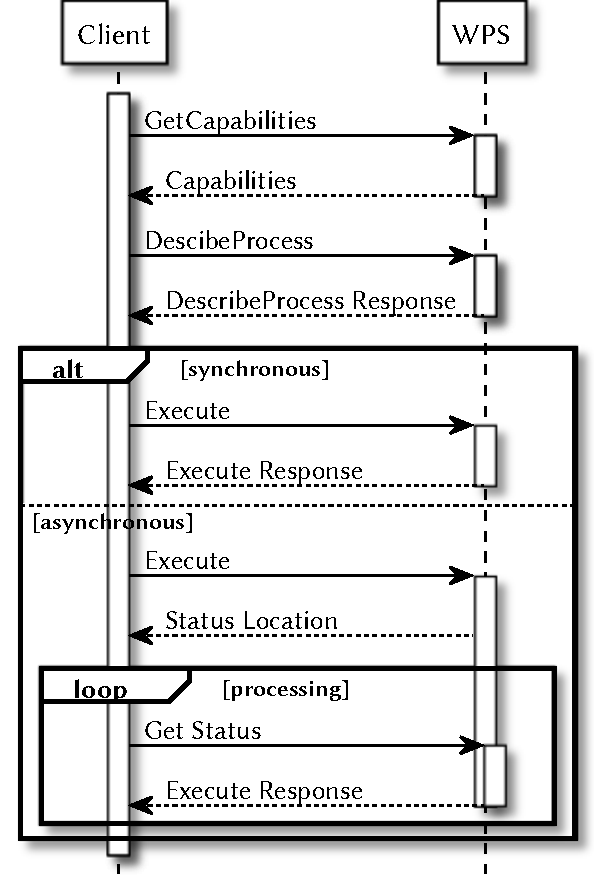
\includegraphics[width=.4\textwidth]{figures/sequence-diagramm-wps.pdf}
		\caption{\label{fig:sd:wps} Typical interaction patterns of the \acl{WPS}. Process discovery using \emph{GetCapabilities} and \emph{DescribeProcess}, synchronous and asynchronous process execution using \emph{Execute}.}
	\end{figure}

	The \ac{WPS} describes three basic types of input and output parameters: \emph{literal}, \emph{complex} and \emph{bounding box} parameters. Complex data parameters are data structures that can be described by a mime type, an encoding and a schema. They can represent raster data, XML structures such as GML feature collections, CSV or any other type of data. This data can be supplied embedded in XML or as a reference to an external HTTP resource. Referenced complex data structures may be requested using HTTP GET or POST and can transport HTTP headers and any body payload (or reference to one). By this chaining of \ac{WPS} processes can easily be implemented, either by referencing a previous generated output or even by encoding another \emph{Execute} call into the reference. Literal data is data, that can be represented by a single string value. The value is described by a data type and can be accompanied by a unit of measurement. Typical data types include single strings, URIs, boolean values, dates and integral or decimal numbers. Bounding box data represents a rectangular region in arbitrary dimension, that is described by a \ac{CRS}.

	TODO: Überleitungssatz zum Matlab-WPS
\section{Matlab WPS}
	\begin{itemize}
		\item closed source, commercial software by The MathWorks, Inc.
		\item high-level language and interactive environment
		\item numerical computation, visualization and programming
		\item origins in matrix computations (\emph{Mat}rix \emph{Lab}oratory)
		\item weakly, dynamical typed language
		\item cross platform
		\item toolboxs
		\begin{itemize}
			\item statistics
			\item curve fitting
			\item neural network
			\item image processing
			\item financial
			\item bioinformatics
			\item signal processing
		\end{itemize}
		\item Matlab Central
		\begin{itemize}
			\item user contributed toolboxes/files/functions/algorithms/etc.
			\item mostly BSD licensed
		\end{itemize}
		\item widespread in academics, engineering and industry
		\item offering a specialized lake-analyzer process not worth the effort
		\item generic solution would have huge benefit
		\item a lot of models implemented in Matlab can become available as WPS processes
		\item offering matlab programs as WPS processes should be easy procedure
		\item domain experts developing models in Matlab may not have extensive programming experience
		\item probably have no experience in developing web services or java code
		\item no switch in languages should be needed
		\item matlab functions with multiple return values
		\item create framework to easily expose a matlab function as an WPS process
		\item requirements
		\begin{itemize}
			\item no web service programming/java programming experience should be needed
			\item pooling of matlab instances to reduce latency
			\item support for WPS complex inputs without dependency to a specific format
			\item existing models and algorithms should be easy (and not intrusive) to expose as WPS algorithms
			\item process description should be manually be written, but be easily generated
			\item
		\end{itemize}
		\item previous approaches: WPS4R
		\begin{itemize}
			\item heavily format specific
			\begin{itemize}
				\item parsing of GML/etc in the WPS and translation to R structures
				\item configuration as comments in R scripts
				\item focussing on scripts and not on functions
			\end{itemize}
		\end{itemize}
	\end{itemize}
	\begin{itemize}
		\begin{figure}[!htb]
			\centering
			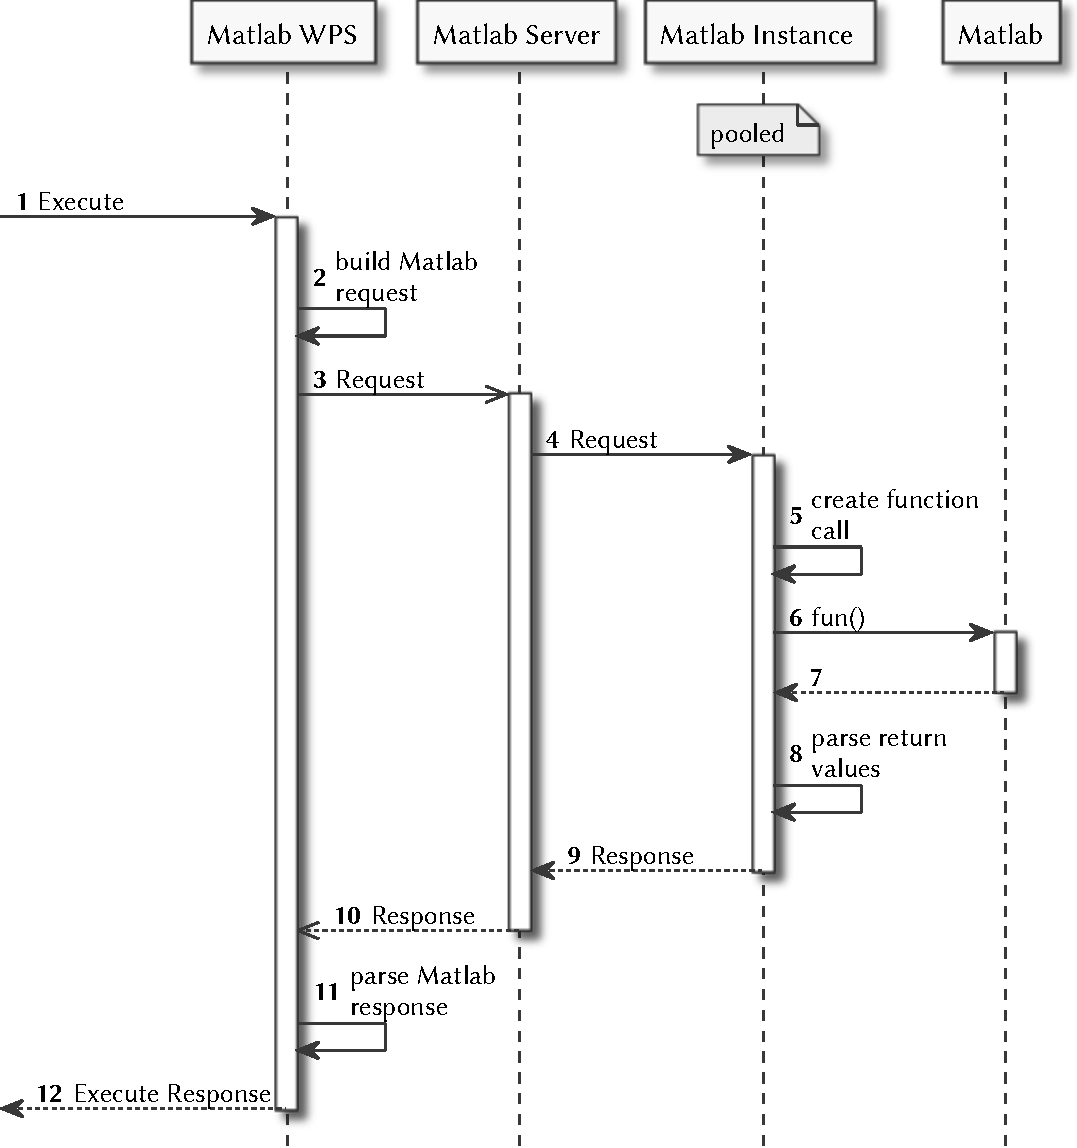
\includegraphics[width=.8\textwidth]{figures/sequence-diagramm-mwps.pdf}
			\caption{\label{fig:sd:mwps} Sequence diagram of the Matlab WPS.} %182x194
		\end{figure}
		\item matlab function <-> wps process
		\item not format specific
		\item no conversion of complex inputs/outputs
		\begin{itemize}
			\item single output formats
		\end{itemize}
		\item matlab program has to parse inputs
		\item easy to publish existing scripts and functions as WPS processes
		\item multi-tier implementation
		\begin{itemize}
			\item Matlab WPS
			\begin{itemize}
				\item Translates WPS Execute requests to Matlab client requests
				\item Translates Matlab client responses to WPS Execute responses
				\item configuration with YAML file to create description and translate inputs/outputs
			\end{itemize}
			\item Matlab Client
			\begin{itemize}
				\item WebSocket client to access the Matlab server.
				\item offers simple request building API
			\end{itemize}
			\item Matlab Server
			\begin{itemize}
				\item WebSocket server that pools multiple Matlab Instances
				\item delegates requests to free instances
			\end{itemize}
			\item Matlab Instance
			\begin{itemize}
				\item a Java wrapper around a Matlab instance
			\end{itemize}
			\item Matlab
			\begin{itemize}
				\item A headless instance of the Matlab software
			\end{itemize}
		\end{itemize}
	\end{itemize}
	\subsection{Configuration}
	\lstinputlisting[label={lst:matlab:example:fun},
					 caption={Matlab example function that represents a simple addition.},
					 float=!htb,language=Matlab]{listings/matlab-add-function.m}
	\lstinputlisting[language=YAML,float=!htb,
					 label={lst:matlab:example:yaml},
					 caption={Matlab process configuration describing the function in Listing \ref{lst:matlab:example:fun}.},
					 morekeywords={function,connection,identifier,version,inputs,outputs,type},
					 morendkeywords={double}]{listings/matlab-add-process-configuration.yaml}
	\lstinputlisting[label={lst:matlab:example:desc},
					 caption={[Process description generated from the configuration in Listing \ref{lst:matlab:example:yaml}.]Process description generated from the configuration in Listing \ref{lst:matlab:example:yaml} (see Appendix \ref{sec:xmlnamespaces} for omitted XML namespaces).},
					 float=!htb,language=XML]{listings/matlab-add-process-description.xml}
	\begin{itemize}
		\item Can not be used to offer any function as process
		\item would not conform to Mathworks license
		\item configuring of a single function as a process
		\item configuration YAML file
	\end{itemize}


	\subsection{Type Mapping}
		\begin{table}[!htb]
			\sffamily\centering
			\caption{\label{tab:matlab:typemapping}Type Mapping between Matlab and WPS Data}
			\begin{tabular}{@{}llcc@{}}
				\toprule
				&
				& \multicolumn{2}{b}{Matlab Type}\\
				\cmidrule(l){3-4}
				\multicolumn{1}{@{}b}{}
				& \multicolumn{1}{b}{Data}
				& \multicolumn{1}{b}{For single inputs}
				& \multicolumn{1}{b@{}}{For multiple inputs}\\
				\cmidrule(rl){2-2}
				\cmidrule(rl){3-3}
				\cmidrule(l){4-4}
				\textbf{Complex}      & \textit{any} & String  & Cell \\\midrule
				\textbf{Bounding Box} & -            & -       & -    \\\midrule
				\textbf{Literal}      & xs:int       & Numeric & Array\\
									  & xs:boolean   & Numeric & Array\\
									  & xs:dateTime  & Numeric & Array\\
									  & xs:double    & Numeric & Array\\
									  & xs:float     & Numeric & Array\\
									  & xs:byte      & Numeric & Array\\
									  & xs:short     & Numeric & Array\\
									  & xs:int       & Numeric & Array\\
									  & xs:long      & Numeric & Array\\
									  & xs:string    & String  & Cell \\
									  & xs:anyURI    & String  & Cell \\
				\bottomrule
			\end{tabular}
		\end{table}
	\subsection{Pooling}
	\begin{itemize}
		\item matlab instances are pooled
		\item reduced starting time of instances
		\item limitation of instances
	\end{itemize}
	\subsection{License Issues}
		\textsc{Matlab} usage is, as any software, restricted by the softwares license. \textsc{Matlab} is a proprietary and commercial product and a such the software and its usage is more restricted than e.g. a open source software such as GNU R. Relevant for the \textsc{Matlab} WPS is section 4.8 of \emph{The MathWorks, Inc. Software License Agreement} \citep{matlablicense}:
		\begin{quote}\itshape
			4. LICENSE RESTRICTIONS.  The License is subject to the express restrictions
			set forth below. Licensee shall not, and shall not permit any Affiliate or any
			Third Party to:
				[...]
				4.8. provide access (directly or indirectly) to the Programs via a web or
				network Application, except as permitted in Article 8 of the Deployment
				Addendum;
		\end{quote}

		As the \textsc{Matlab} WPS offers \textsc{Matlab} functionalities through a web service interface, the usage is highly restricted, as the referenced \emph{Deployment Addendum} \citep{matlablicense} states:

		\begin{quote}\itshape
			8. WEB APPLICATIONS.  Licensee may not provide access to an entire Program or a substantial portion of a Program by means of a web interface.

			For the Network Concurrent User Activation Type.  Programs licensed under the Network Concurrent User Activation Type may be called via a web application, provided the web application does not provide access to the MATLAB command line, or any of the licensed Programs with code generation capabilities.  In addition, Licensed Users may not provide access to an entire Program or a substantial portion of a Program.  Such operation of an application via a web interface may be provided to an unlimited number of web browser clients, at no additional cost, for Licensee's own use for its Internal Operations, and for use by Third Parties.

			For the Network Named User and Standalone Named User Activation Types. Programs licensed under the Network Named User and Standalone Named User Activation Types may be called via a web application, provided the web application does not provide access to the MATLAB command line, or any of the licensed Programs with code generation capabilities, and such application is only accessed by designated Network Named User or Standalone Named User licensees of such Programs.

			Programs licensed under any other Activation Type may not be called via a web interface.
		\end{quote}

		Only the \emph{Network Concurrent User Activation Type} is allowed to offer \textsc{Matlab} scripts and functions as long it does not offer access to the \textsc{Matlab} command line interface. \emph{Network and Standalone Named User} license types require additional authentication mechanism in place in order to restrict the access to the web application. As the \textsc{Matlab} WPS does not offer the possibility to access the \textsc{Matlab} command line interface or substantial portion of \textsc{Matlab}, but restricts access to configured \textsc{Matlab} function calls, customers owning a license of the first type are allowed to deploy a \ac{WPS} offering \textsc{Matlab} processes to a open network, while users of the second class of licenses are still allowed to deploy them with an additional authentication mechanism. Using a pool of \textsc{Matlab} instances on a remote server on the other hand introduce additional problems in regard of the license. In theory these \textsc{Matlab} can be used to perform about any function call, and thus provide access to the \textsc{Matlab} command line interface. Even though the access is restricted to simple function calls and does not allow variable declaration, nested function calls or function definition, it may be considered a license violation the deploy this infrastructure in a public environment.

		A conclusive analysis of the legal implications of the system is out of the scope of this thesis, but certainly should be done before a system facilitating the \textsc{Matlab} WPS or any of its components is deployed in a public or productive environment.
	\subsection{Implementation}

	\subsection{Lake-Analyzer WPS}
\section{Streaming WPS}
	% dataset vs. data set
	In contrast to conventional data processing, such as the method used in the \ac{WPS}, streaming processing approaches show considerable benefits. Regarding to time efficiency and with reference to the already mentioned problems of processing substantial large data sets or live data, the development of a streaming enabled \ac{WPS} seems to be of great value.

	Data streams describe a abstract concept that stands in contrast to conventional batch data. Data streams are (possibly infinite) sequences of data items (or chunks), that become available over time, while conventional batch data describes a pile of data, that is either completely available or not. The abstract concept of streaming can be observed across different technologies and fields of application. Starting from the concept of pipes and filters on unix-like operation systems, over interprocess communications using sockets \citep[either local or over a network,][]{buschmann1996pattern}, the ubiquitous usage in programming languages (as a concept of I/O or in functional programming languages in the form of inductive data type definitions), over \ac{GPGPU} to modern media streaming solutions like RTP and RTCP \citep{ietf:rfc3550}, RTSP \citep{ietf:rfc2326} or SIP \citep{ietf:rfc3261}.
	The concept can be best shown on it's most popular usage form: media streaming. The conventional approach to view a video or play a sound file over a network is to download the file and to play it locally. Depending on the coding/compression format used to encode the media file, it is not possible to play the file until the download is finished. Media streaming reduces time to start playing drastically by sending smaller parts of the media file over the network (e.g. one or more single frames). Suitable player are now able to play this stream of frames long before the complete file is transmitted. Besides th on-demand streaming of media (the streamed file is completely available on the remote side), the transmission of live audio or video becomes possible by transferring audio/video frames as soon as they are recorded.

	The concept of streaming processing extends this simple pattern by not only accepting a stream of input data, but also by generating a stream of output data. The processing takes place on small chunks of the input data instead of the complete data set. By sequentially processing the stream programs are able to process very large or infinite datasets, because the complete dataset neither needs to be kept in memory nor it is needed to be stored. This permits the analysis of live data, e.g. the evaluation of continuously collected sensor data. Also the initial response time (the time until the first outputs of a program are available) is equally reduced as in media streaming. Reducing the latency of initial data output has various advantages, e.g. earlier appearance of errors (and by this the possibility to stop processing to save computing resources and time) or the ability to develop more responsive end user solutions, e.g. by gradually updating a data visualization instead of presenting the data after waiting for the complete result.

	In the case of spatiotemporal data, streaming processing is especially useful and advisable, as datasets tend to become rather large and the analysis of real-time data can have great benefits, especially as spatiotemporal data is often an ideal candidate to streaming, as spatial data sets are often aggregates or collections, that can be easily broken down into smaller parts (like single features, observations or tiles). On the other side spatiotemporal data has the salient characteristic of showing strong dependencies to nearby data and thus can be difficult to analyze using non-random-access paradigms like streaming. The case of inter-feature dependencies has to especially considered when transferring the concept of streaming to spatiotemporal processing. Algorithms used in streaming are required to operate on smaller chunks of the complete dataset and computations, that require global knowledge are not expected any advantage from streaming. E.g. graph algorithms like Dijkstra's algorithm \citep{dijkstra} can not start the computation before the complete graph is available.

	Streaming processing can be divided into three categories, that differ from conventional processing (see Figure \ref{fig:streaming} (a)). Characteristic for input streaming (b) is the parallel occurrence of input and processing with a subsequent output after processing finished. On the other hand, output streaming processing describes the isolated input supply and parallel processing and output (c). Combining these two approaches results in the third category, full input and output streaming, in which input, processing and output take place concurrently. Despite their respective concurrency, all three categories have the very same advantage. By parallelizing processing and input and/or output, the overall execution and initial response time is appreciably shorter. Full input and output streaming enabled processes have the additional advantage to be able to process indefinite large datasets by processing each input data chunk separately and outputting a output data chunk for each of them. Through this the analysis of live sensor data can be accomplished.
	Each of these categories of processing demands different requirements from the process or algorithm. To create a stream the dataset needs to divisible into smaller chunks, input streaming enabled algorithms need to be able to operate on each of these chunks separately and output streaming enabled processes need to be able to produce intermediate results. Input streaming would result in no benefits for algorithms requiring global knowledge of the dataset, because they can not start processing prior to all data chunks have arrived. Processes that result in a single output value, for which the processing has to be completed offer no advantage, when they are output streaming enabled.

	\begin{figure}[!htb]
		\centering
		% !TEX root = ../thesis.tex
\begin{tikzpicture}
	\scriptsize
	\tikzset{
	  ibox/.style = {draw, fill=string!50,  minimum width=4cm, minimum height=.6cm},
	  pbox/.style = {draw, fill=comment!50, minimum width=4cm, minimum height=.6cm},
	  obox/.style = {draw, fill=keyword!50, minimum width=4cm, minimum height=.6cm},
	  every node/.style={font=\sffamily},
	}
	\draw[>->] (-2.4,3.6) -- (11.4,3.6);
	%\draw[]   (-2.4,3.6) -- (-2.4, -6);
	\draw[>->] (-2.4, -6) -- (11.4, -6);

	\draw[dotted] (-2.0,-6) -- (-2.0,3.6);
	\draw[dotted] (-1.0,-6) -- (-1.0,3.6);
	\draw[dotted] (-0.0,-6) -- (-0.0,3.6);
	\draw[dotted] (1.0,-6) -- (1.0,3.6);
	\draw[dotted] (2.0,-6) -- (2.0,3.6);
	\draw[dotted] (3.0,-6) -- (3.0,3.6);
	\draw[dotted] (4.0,-6) -- (4.0,3.6);
	\draw[dotted] (5.0,-6) -- (5.0,3.6);
	\draw[dotted] (6.0,-6) -- (6.0,3.6);
	\draw[dotted] (7.0,-6) -- (7.0,3.6);
	\draw[dotted] (8.0,-6) -- (8.0,3.6);
	\draw[dotted] (9.0,-6) -- (9.0,3.6);
	\draw[dotted] (10.0,-6) -- (10.0,3.6);
	\draw[dotted] (11.0,3.6) -- (11.0,-6) node [below] {Time};

	\node [xshift=-1.5cm,yshift=2.4cm] {(a)};
	\node [ibox,yshift=3.0cm,xshift=1cm] (input1) {Input Upload};
	\node [pbox,yshift=2.4cm,xshift=5cm] (processing1) {Processing};
	\node [obox,yshift=1.8cm,xshift=9cm] (output1) {Output Download};

	\draw[dashed] (-2.4, 1.2) -- (11.4, 1.2);

	\node [xshift=-1.5cm,yshift=0cm] {(b)};
	\node [ibox,yshift= .6cm,xshift=1cm] (input2) {Input Stream};
	\node [pbox,yshift= .0cm,xshift=2cm] (processing2) {Processing};
	\node [obox,yshift=-.6cm,xshift=6cm] (output2) {Output Stream};

	\draw[dashed] (-2.4, -1.2) -- (11.4, -1.2);

	\node [xshift=-1.5cm,yshift=-2.4cm] {(c)};
	\node [ibox,yshift=-1.8cm,xshift=1cm] (input3) {Input Stream};
	\node [pbox,yshift=-2.4cm,xshift=5cm] (processing3) {Processing};
	\node [obox,yshift=-3.0cm,xshift=6cm] (output3) {Output Stream};

	\draw[dashed] (-2.4, -3.6) -- (11.4, -3.6);

	\node [xshift=-1.5cm,yshift=-4.8cm] {(d)};
	\node [ibox,yshift=-4.2cm,xshift=1cm] (input4) {Input Stream};
	\node [pbox,yshift=-4.8cm,xshift=2cm] (processing4) {Processing};
	\node [obox,yshift=-5.4cm,xshift=3cm] (output4) {Output Stream};
\end{tikzpicture}
		\caption{\label{fig:streaming}Four different types of processing data: (a) conventional processing, (b) streaming input data (c) streaming output data, (d) full input and output streaming \citep[based on][]{foerster2012live}.}
	\end{figure}

	While there are efforts to utilize popular techniques like grid and cloud computing, there are few efforts in research and development to facilitate streaming processing \citep{foerster2012live}. Previous approaches to combine the concept of streaming and web-based processing of spatiotemporal data using the \ac{WPS} are drafted in strong correlation to media streaming \citep{foerster2012live} by using playlist files \citep{ietf:draft-pantos-http-live-streaming-12} as inputs and outputs of a \ac{WPS} process. The process is executed asynchronously and the output playlist location is published using the \texttag{wps}{ProcessStarted} element of the process status response (see Figure \ref{fig:sd:previous}). As the \ac{WPS} specification is not designed to be extensible, the elements content is restricted to a simple string and can not contain complex \ac{XML} structures. Furthermore the elements definition states, that it should used to convey a human readable text that is presented to an user:
	\begin{signedquote}{\cite{ogc:wps}}
		A human-readable text string whose contents are left open to definition by each WPS server, but is expected to include any messages the server may wish to let the clients know. Such information could include how much longer the process may take to execute, or any warning conditions that may have been encountered to date. The client may display this text to a human user.
	\end{signedquote}
	Despite the goal of maintaining compatibility to \ac{WPS} specification and existing software components, this represents a misappropriation of the element and will result in incompatibilities with existing \ac{WPS} client solutions. Besides that, this solution is only able to transport a single playlist location to the client and thus, a \ac{WPS} process may only have a single streaming output.

	\begin{figure}[!htb]
		\centering
		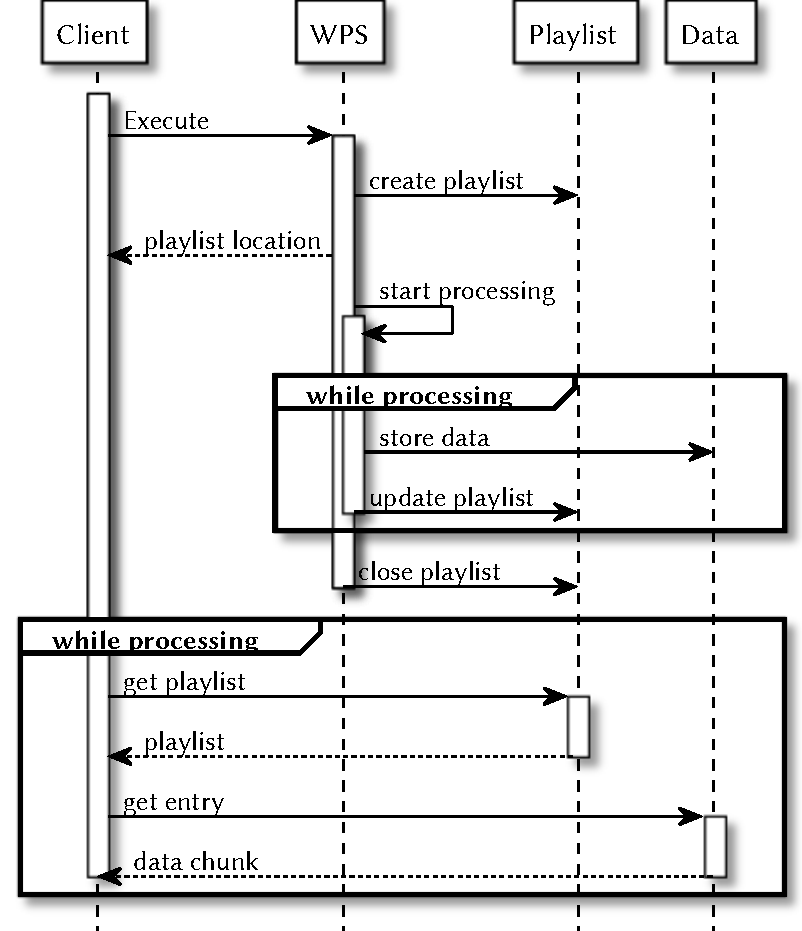
\includegraphics[width=.6\textwidth]{figures/sequence-diagramm-previous.pdf}
		\caption{\label{fig:sd:previous} Sequence diagram of the playlist-based streaming enabled WPS \citep{foerster2012live}.}
	\end{figure}

	Input parameters may also be supplied using a playlist file. The coordination of several streaming inputs is either not possible or heavily dependent on the streaming enabled process. A process accepting two streamed datasets, that are combined during processing, has to decide which data chunks it has to combine and \dots. Even in the simplest case of combining chunks of both streams with the same index can have serious implications in the use case of live analysis. If a data chunk gets lost, the process, either due to hardware or network failure, the process will combine chunks, that are not related. In continuous process, this error can not be detected, as to indefinite streams of data will always have matching indexes. Use cases in which the rate of incoming data between streams differ or data chunks depend on other chunks are very hard to model and will result in highly specialized processes, that
	depend not only on the structure and format of input data, but also on the data source, and thus it's incoming rate. By this, generic solutions, that convert existing \ac{WPS} processes into streaming enabled processes are hard to develop, and most streaming enabled processes may not be used in contexts other that it was developed for.

	Moreover, realizing streaming by continuous polling of playlists is highly inefficient. Neither can the client know the rate output data is produced nor can the \ac{WPS} process know at which rate input data becomes available. By polling at a too slow rate the arrival of data chunks may be missed, which results in a slower process execution and by polling at a too high rate, network and computation resources are wasted. Adaptive polling rates may be a solution for this problem, but are useless in cases, where the rate of incoming data changes across the process execution. The usage of playlist to transport data from the client to the server, in contrast to transporting data from the server to the client, for which the origin in media streaming playlist was developed, is additionally questionable. Clients need the capability to publish files as resources, that a accessible using a URL (e.g. on a FTP or HTTP server). In a web browser environment, a JavaScript client is only able to do this using an external service, that has to store the data and maintains the playlist. A pure JavaScript browser client is not able to use streaming inputs in this playlist-based streaming \ac{WPS} approach. The implementation of this approach is additionally limited. Input parameter data streams are not implemented and process implementations have to split inputs to create output streams (see Figure \ref{fig:streaming} (c)). Splitting spatiotemporal data into smaller chunks is not as trivial as e.g. splitting a audio or video stream in single frames and so the process implementations become heavily format dependent and dependencies between data chunk can only expressed as part of the data, in a format, that the process is able to understand and to handle. Also this approach requires a reimplementation of already existing processes to achieve streaming outputs.

	% TODO: daten hängen von ihrer umgebung ab: quelle?
	A streaming enabled \ac{WPS} should extend the traditional processing paradigm (see Figure \ref{fig:streaming} (a)) to enable input only streaming (Figure \ref{fig:streaming} (b)), output only streaming (Figure \ref{fig:streaming} (c)), and full input/output streaming (Figure \ref{fig:streaming} (d)), for which input parameters are supplied subsequently and output data chunks is published as it becomes available. To accomplish this, it should not rely on inefficient polling techniques, in which the server or client is requesting a resource continuously over time, but should rely on true streaming technologies, that offer a full-duplex communication channel between client and server. Streaming enabled process should be accessible from the same environments as conventional \ac{WPS} processes. This especially includes web browser environments, that are particular restricted in their possibilities. A streaming enabled \ac{WPS} process should rely on existing widely known and standardized technologies, it should be especially as interoperable as possible to the \ac{WPS} specification, but should not compromise streaming functionality by enforcing incompatible standards. As spatiotemporal and it's processing and analysis often can not be treated independent to surrounding data, dependencies between streamed data chunks have to be considered. This will require the streaming enabled process to be able not only to operate on sequential data but also be able to allow, to some degree, random access to the data. Despite handling of dependencies between spatiotemporal features should be considered, processes and algorithms, that require global knowledge of the dataset may not profit from a streaming enabled WPS and should not be considered relevant for a streaming enabled \ac{WPS}. The system should be as generic as the existing \ac{WPS} specification, so it should not rely on specific data formats and allow easy chaining of streaming processes. As possible use cases include not only live analysis of data, but also the processing of large dataset, data chunks should be processed in parallel if possible. As this may result in a undefined order of outputted data chunks, client need to be able to correlate output data chunks with the input parameter chunks. Existing \ac{WPS} processes should be easily converted to streaming enabled processes, without the need to develop them from scratch.

	The following sections should introduce a approach for a Streaming \ac{WPS}, that will fulfill the above requirements. As seen in previous approaches the constraints imposed by the \ac{WPS} specification are too strict to implement a streaming enabled WPS fulfilling the requirements, that is compatible to the standard. Previous solutions compromised functionality for sake of (incomplete) compatibility with the inflexible standard. In order to enable true, browser compatible, streaming this approach will break out of the constraining \ac{WPS} standard and develop a message based architecture using WebSockets to accomplish true full-duplex streaming of data while reusing terminology and technology specified by the \ac{WPS} specification.

\subsection{Protocol}
	As the the \ac{WPS} specification is not flexible enough to model a full streaming scenario, the \ac{WPS} has to be bypassed. For this a more flexible interaction model was developed, that extends the conventional processing approach. This protocol is message based and enables full-duplex stream processing of spatiotemporal data. A \emph{streaming enabled algorithm} is a \ac{WPS} algorithm that supports the here defined protocol while a \emph{streaming process} is the identifiable instance of an algorithm, created by executing the streaming enabled algorithm using the \ac{WPS} Execute operation. The streaming process is the core of the Streaming \ac{WPS} and receives subsequent inputs and will emit intermediate results. While the execution of the streaming enabled algorithm is fully supported by the \ac{WPS} specification, all interaction with the streaming process is not part of the standard. To communicate with the streaming process, the client needs information on how to connect to the process. As the \ac{WPS} specification does not allow subsequent outputs, the call of the Execute operation will return immediately to transport this information to the client, and can not persist over the lifetime of the streaming process.

	To enable a full duplex communication with the streaming process WebSockets will be used to transport messages. This is needed to \emph{push} messages to clients instead of letting the clients constantly request updates.

	\begin{figure}[!htb]
		\centering
		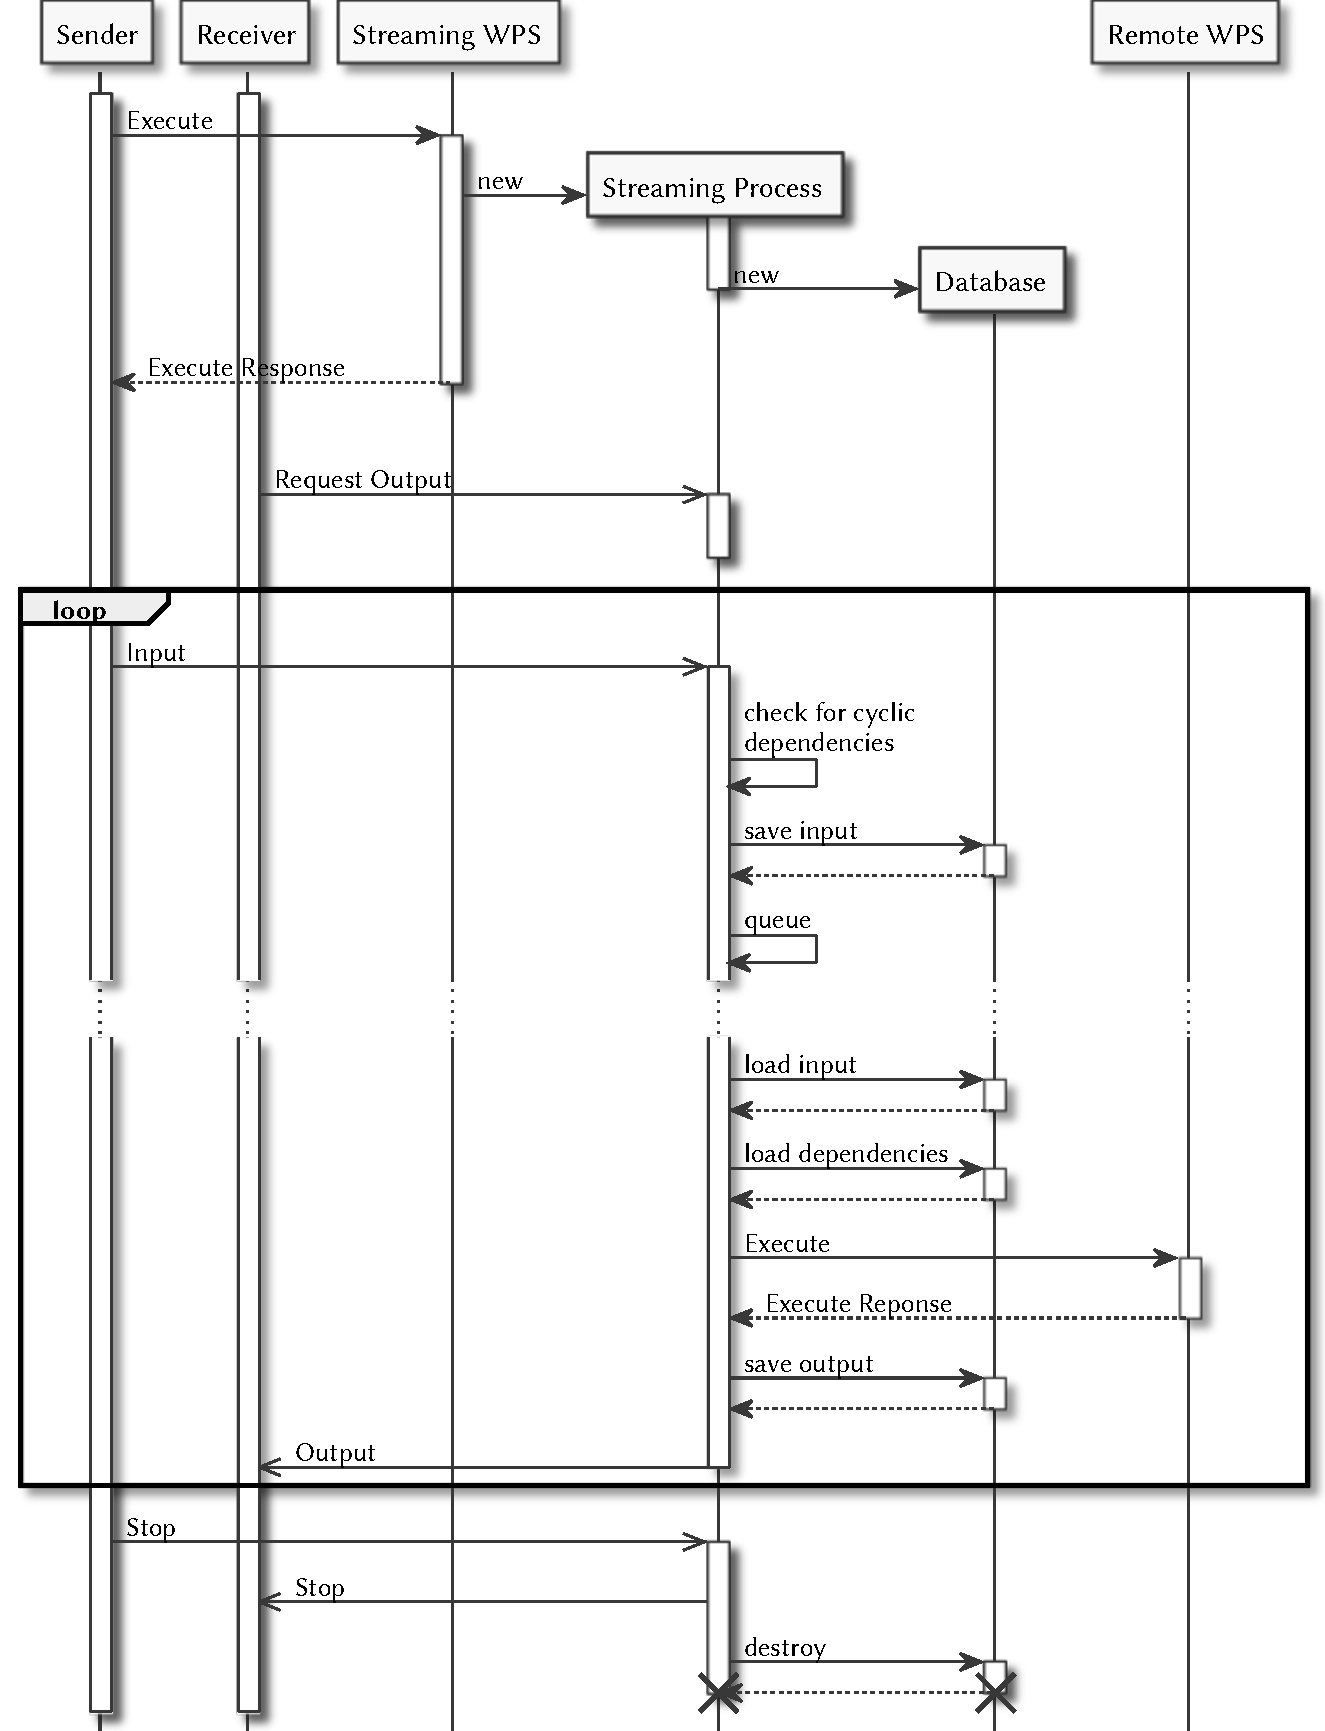
\includegraphics[width=.7868\textwidth]{figures/sequence-diagramm-swps.pdf} % 179x274
		\caption{\label{fig:sd:swps} Sequence diagram of typical interaction pattern with a streaming enabled WPS algorithm using two distinct clients for sending and receiving data.}
	\end{figure}

	The detailed interaction protocol is depicted in Figure~\ref{fig:sd:swps}. A client (\emph{Sender}) issues a Execute to a streaming enabled WPS algorithm (\hyperref[fig:sd:swps]{step 1}). The algorithm will instantiate a delegate (\hyperref[fig:sd:swps]{step 2}), that is responsible for processing data chunks, and a streaming process (\hyperref[fig:sd:swps]{step 3}), that is responsible for client interactions and task scheduling. The Execute response will contain the necessary details to connect to the streaming processes, such as the the identifier of the streaming process and the WebSocket endpoint URL (\hyperref[fig:sd:swps]{step 4}).

	With these details a client can connect directly to the streaming process bypassing the \ac{WPS} interface. In \hyperref[fig:sd:swps]{step 5} another client\footnote{Even though sender and receiver are two different entities in this diagram, there are no restrictions imposed to the amount of clients, either senders or receivers, or their nature (senders may also be receivers).} (\emph{Receiver}) connects to the streaming process and subscribes to the future outputs of the process. By this the client does not need to constantly issue requests to the streaming process to check for new outputs, but will receive outputs automatically as long as the receiving client stays connected using the WebSocket.
	After this one or multiple clients start sending chunks of data as input parameters to the streaming process (\hyperref[fig:sd:swps]{step 6}). The clients may open a new connection for every input or use the same connection over the lifetime of the streaming process. The streaming process will check the inputs for validity (\hyperref[fig:sd:swps]{step 7}) and will queue them for processing (\hyperref[fig:sd:swps]{step 8}).
	Processing takes places asynchronously in parallel manner and there is no guarantee of order (besides restrictions imposed by dependencies, see sections \ref{sec:stream:input:reference} and \ref{sec:stream:dependencies}). When there are free capacities to process the data and all other requirements are met, the delegate will be tasked to process the data (\hyperref[fig:sd:swps]{step 9}). The delegate implementation can return a intermediate result in \hyperref[fig:sd:swps]{step 10}, which will be forwarded to all registered receivers in \hyperref[fig:sd:swps]{step 11}.
	Steps 6 to 11 may be repeated indefinitely (e.g. live analysis of data) or until the sending client has no more inputs to feed. As the streaming process would wait in this case for ever (or at least until some timeout interferes), the client has to stop the streaming process explicitly (\hyperref[fig:sd:swps]{step 12}).
	This will cause the streaming process to stop accepting inputs, to process all not yet processed inputs and to request a last potential output from the delegate (\hyperref[fig:sd:swps]{step 13 \& 14}), which will be forwarded to all listening clients (hyperref[fig:sd:swps]{step 15}). After this it will destruct the delegate (\hyperref[fig:sd:swps]{steps 16 \& 17}) and will notify all registered listeners, that there will be no further outputs become available by publish forwarding the stop message (\hyperref[fig:sd:swps]{step 18}). The streaming process will destroy itself after this.

	A detailed description of the various messages of this protocol can be found in section~\ref{sec:streaming:messages}.

	The protocol permits various streaming usage scenarios. A delegate, that produces a output for every input message creates a full input/output streaming process (see Figure~\ref{fig:streaming} (d)), a delegate that produces only a final output results in a input only streaming process (see Figure~\ref{fig:streaming} (b)). By suppling a single input message and repeating step 11, a suitable delegate may create a output streaming process (see Figure~\ref{fig:streaming} (c)) and, although not reasonable, even the traditional processing approach depicted in Figure~\ref{fig:streaming} (a) can be simulated by passing all inputs in a single input message and producing a single output message.

	Using message provoked streaming iterations (the combination of a input message, its processing and (optional) output message) allows the use of multiple streaming inputs and outputs. In contrast to previous approaches it is possible for the streaming process to relate these to a single processing iteration without any knowledge of their semantics, because the client encapsulates them in a single message.

	\begin{figure}[!htb]
		\centering
		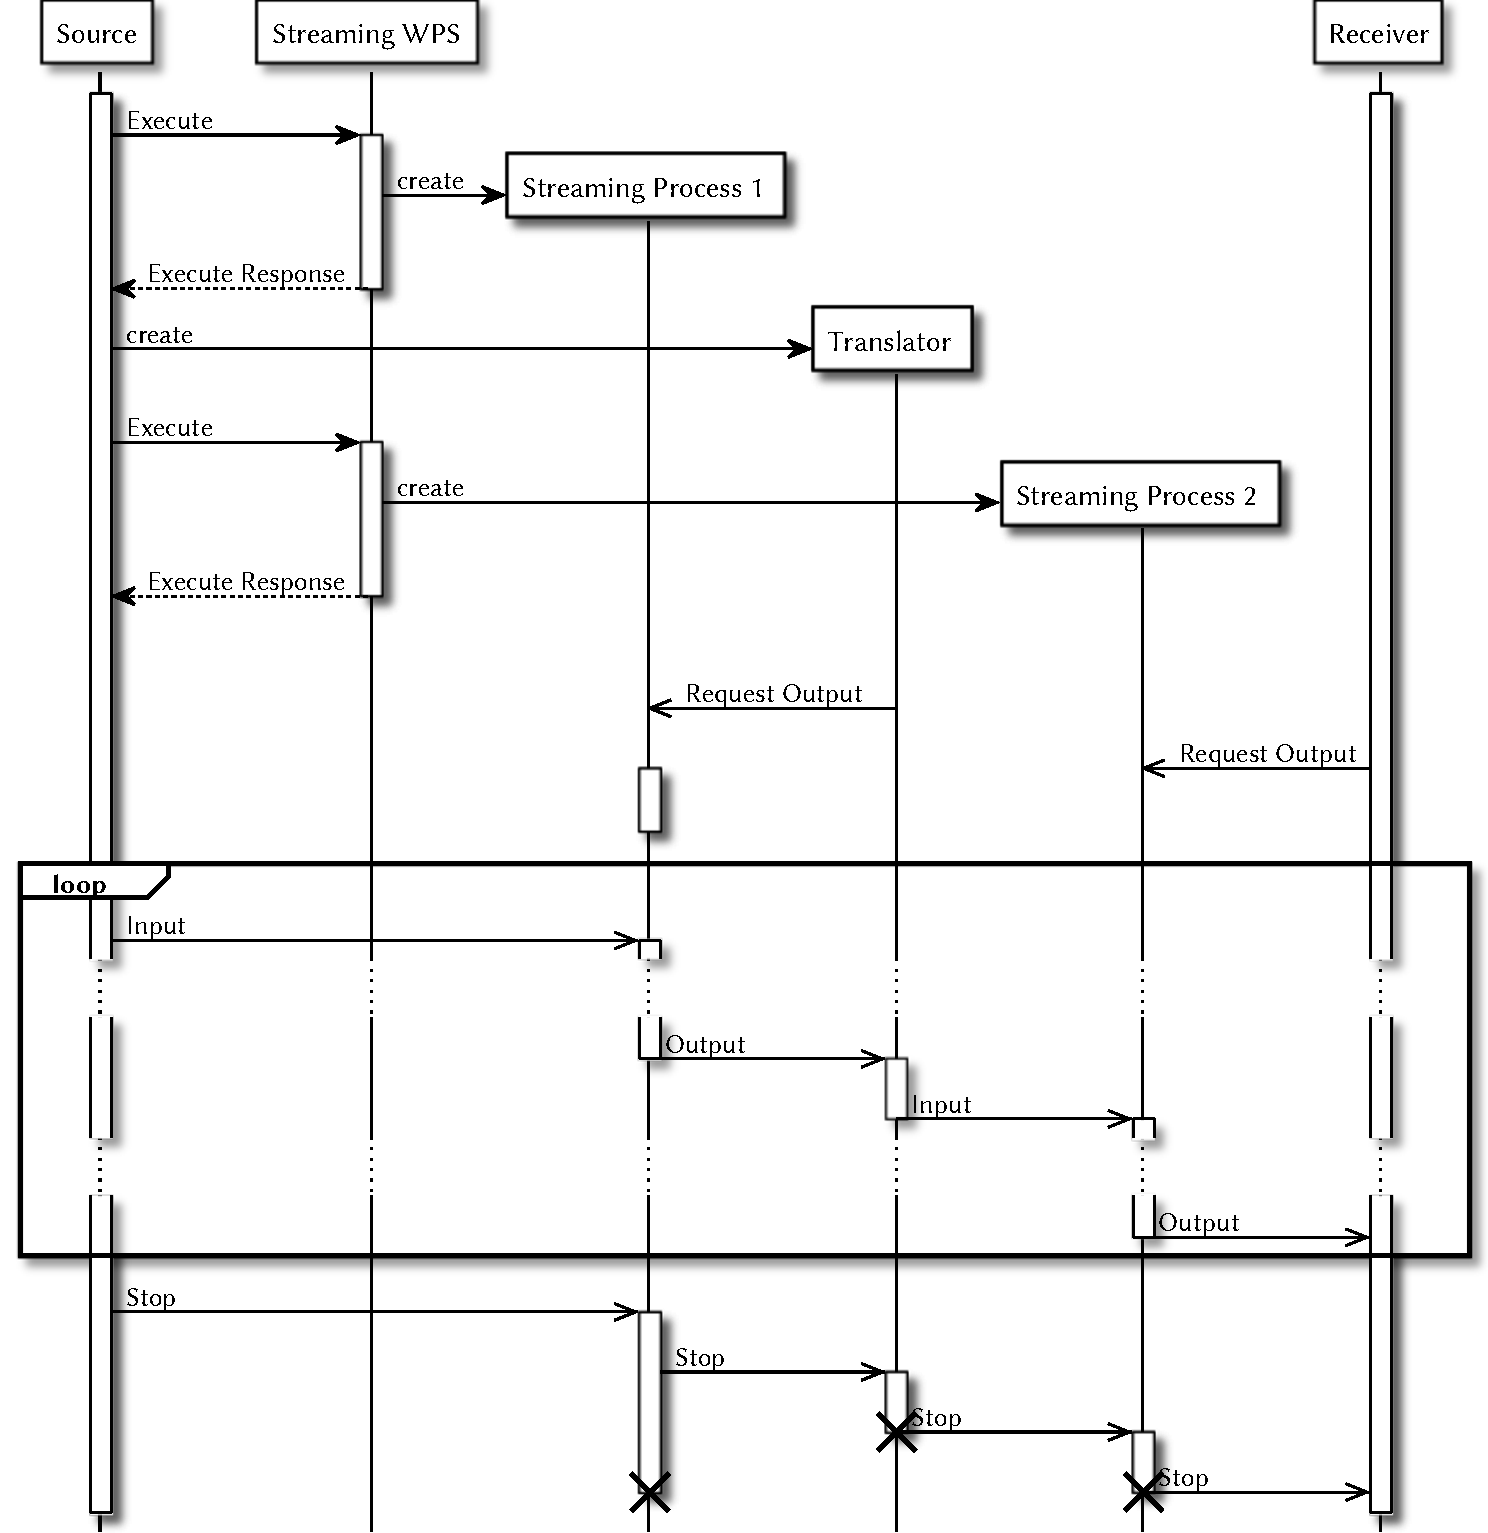
\includegraphics[width=\textwidth]{figures/sequence-diagramm-chain.pdf} % 179x274
		\caption{\label{fig:sd:chain} Sequence diagram of chaining two streaming processes using a generic mediator between the processes to translate output to input messages.}
	\end{figure}

	The protocol also enables the chaining of processing steps. This can be realized in two ways: a delegate itself may represent a \ac{WPS} process chain and thus chain every processing step or several streaming process are chained itself. A simple mediator translating input messages to output messages (see Figure~\ref{fig:sd:chain}). This mediator can be realized using a dedicated streaming enabled algorithm accepting a input/output mapping and the connection parameters of the streaming processes to connect. After requesting the outputs of the source streaming process it can translate every output message to an input message and forward the stop message. A receiving client will simply connect to the second streaming process and will received the data process by the chain. By requesting the outputs first streaming process even intermediate result of the chain are accessible.

	\subsection{Messages}
		\label{sec:streaming:messages}
		To fulfill the above defined protocol several messages have to be exchanged between sender, streaming process and receiver. In order to correlate input and outputs or to show the source of an error, the message format has to have a concept of message references. WebSockets do not have such a concept as it is only a thin layer on top of TCP, that introduces handshake and addressing mechanism to be compatible with HTTP and a minimal framing of messages. This framing is merely needed to establish a message-based instead of a stream-based protocol, as the latter would make it hard to differentiate between individual messages \citep{ietf:rfc6455}. To enable referencing of messages, and by this a asynchronous reply mechanism, another layer is needed. As the \ac{WPS} is mostly based on \ac{XML}, the message format should also be \ac{XML} based. This enables the usage of large parts of the \ac{WPS} schema and allows the reuse of many components written to interact with the \ac{WPS}.

		The widely known SOAP protocol \citep{w3c:soap1}, which may also be used as an optional binding of the \ac{WPS} and thus can be easily adopted, is a ideal candidate for this. In combination with \ac{WSA} \citep{w3c:wsa} it creates a \ac{XML} based message framework, that allows asynchronous requests and responses over a arbitrary protocol. Besides introducing a concept of addressing and routing of messages (that will not be used in the Streaming \ac{WPS}), one can assign a globally unique identifier to any message using \ac{WSA}, that can be referenced with arbitrary semantics (e.g. reply).

		The Streaming \ac{WPS} defines seven SOAP messages.

		\paragraph{Input Message}
			Input messages are used by clients to supply subsequent inputs to a streaming iteration of a streaming process. They loosely resemble a \ac{WPS} Execute request by consisting of any number of inputs and a identifier, which references the streaming process to which the inputs should be supplied. An example can be seen in Listing \ref{lst:streaming:message:input}, possible inputs can be seen in section \ref{sec:streaming:input}.
			\lstinputlisting[label={lst:streaming:message:input},
			                 caption={[Example for a Streaming WPS input message.]Example for a Streaming WPS input message (see Appendix \ref{sec:xmlnamespaces} for omitted XML namespaces).},
			                 float=!htb,language=XML]{listings/streaming-message-input.xml}
		\paragraph{Output Messages}
			Output messages are used by the streaming process to transport intermediate results at the end of a streaming iteration or a final result at the end of the streaming process to listening clients. They loosely resemble a \ac{WPS} Execute response by containing a arbitrary number of outputs and the identifier of the process, that produced the outputs. Output messages containing intermediate result are replies to their corresponding input message and reference them using \ac{WSA}. If the processing used the output of any other streaming iteration (see sections \ref{sec:stream:input:reference} and \ref{sec:stream:dependencies}) the corresponding output messages are also referenced. An example can be seen in Listing \ref{lst:streaming:message:output}.
			\lstinputlisting[label={lst:streaming:message:output},
			                 caption={[Example for a Streaming WPS output message.]Example for a Streaming WPS output message (see Appendix \ref{sec:xmlnamespaces} for omitted XML namespaces).},
			                 float=!htb,language=XML]{listings/streaming-message-output.xml}
		\paragraph{Output Request Message}
			A output request message is used by client to let a streaming process know, that it would like to receive outputs from the process. There is no direct counter part in the \ac{WPS} specification but the concept is similar to the continuous request of the \ac{WPS} response during a asynchronous process execution. As WebSockets offer a full-duplex messaging channel a continuous polling of outputs is not needed, but the streaming process can push outputs directly to listening clients. To initialize this listening the client register to one or more streaming processes using their corresponding identifiers. An example can be seen in Listing \ref{lst:streaming:message:output-request}.
			\lstinputlisting[label={lst:streaming:message:output-request},
			                 caption={[Example for a Streaming WPS output request message.]Example for a Streaming WPS output request message (see Appendix \ref{sec:xmlnamespaces} for omitted XML namespaces).},
			                 float=!htb,language=XML]{listings/streaming-message-output-request.xml}
		\paragraph{Stop Message}
			As streaming process can run indefinitely long, input supplying clients need to be able to let the streaming process know, that there will be no further inputs become available. To achieve this a stop message (see Listing \ref{lst:streaming:message:stop}) is send to the streaming process. The process will propagate the stop message to all listening clients to let them know there will be no further outputs. Before the stop message is propagated all streaming iterations, that are not yet processed will be finished but the process will not accept any further inputs. If there are still unresolved dependencies (see sections \ref{sec:stream:input:reference} and \ref{sec:stream:dependencies}) the streaming process will fail with an error message.
			\lstinputlisting[label={lst:streaming:message:stop},
			                 caption={[Example for a Streaming WPS stop message]Example for a Streaming WPS stop message (see Appendix \ref{sec:xmlnamespaces} for omitted XML namespaces).},
			                 float=!htb,language=XML]{listings/streaming-message-stop.xml}
		\paragraph{Error Message}
			Errors are transported, as in the \ac{WPS} specification, using \ac{OWS} exception reports \citep{ogc:wps}. If the delegate of a process fails or a supplied input message can not be processed due to whatever conditions, the error is propagated to listening clients. The error is always send to the client that send the message causing the error (if the client is still connected) and in case the error is caused during the execution of a streaming iteration also to all listening clients, that registered through a output request message. In contrast to failures during input validation, due to constraints imposed by dependencies (see sections \ref{sec:stream:input:reference} and \ref{sec:stream:dependencies}), errors raised during the execution of a streaming iteration can not be compensated, but will stop the streaming process. The causing message of a failure may obtained from the reply relation encoded using \ac{WSA}. An example of an error message can be found in Listing \ref{lst:streaming:message:error}.
			\lstinputlisting[label={lst:streaming:message:error},
			                 caption={[Example for a Streaming WPS error message.]Example for a Streaming WPS error message (see Appendix \ref{sec:xmlnamespaces} for omitted XML namespaces).},
			                 float=!htb,language=XML]{listings/streaming-message-error.xml}
		\paragraph{Describe \& Description Message}
			Describe messages are directly adopted from the \ac{WPS} Describe Process operation. Due to conditions described in section \ref{sec:stream:processdescription} a client needs to able to retrieve a description from a running streaming process. The message simply contains the identifier of the process the clients wants to have the description from (an example can be seen in Listing \ref{lst:streaming:message:describe}).
			\lstinputlisting[label={lst:streaming:message:describe},
							 caption={[Example for a Streaming WPS describe message.]Example for a Streaming WPS describe message (see Appendix \ref{sec:xmlnamespaces} for omitted XML namespaces).},
							 float=!htb,language=XML]{listings/streaming-message-describe.xml}
			The reply resembles a Describe Process response and is encoded in a description message referencing the describe message and containing the streaming process description and (see Listing \ref{lst:streaming:message:description}).
			\lstinputlisting[label={lst:streaming:message:description},
							 caption={[Example for a Streaming WPS description message.]Example for a Streaming WPS description message (see Appendix \ref{sec:xmlnamespaces} for omitted XML namespaces).},
							 float=!htb,language=XML]{listings/streaming-message-description.xml}

	\subsection{Input Types}
		\label{sec:streaming:input}
		The aforementioned requirements imply three different types of input for a Streaming Process. They differ in the aspect of time (\emph{When are they supplied?}) and scope (\emph{Where are they used?}). Besides that all of them are based on the very same input types the \ac{WPS} standard defines (see section \ref{sec:wps}).
		\subsubsection{Streaming Inputs}
			\label{sec:streaming:input:streaming}
			The first and most obvious type of input are streaming inputs. They are provided for a single streaming iteration and will only be used in that iteration representing the core of streaming enabled processing (see Listing \ref{lst:streaming:input:streaming}).

			\lstinputlisting[label={lst:streaming:input:streaming},
			                 caption={[Example for a Streaming WPS streaming inputs.]Example for a Streaming WPS streaming inputs (see Appendix \ref{sec:xmlnamespaces} for omitted XML namespaces).},
			                 float=!htb,language=XML]{listings/streaming-input-streaming.xml}


			A conventional algorithm to compute the histogram of a raster (e.g. a satellite image) needs the complete raster as a single complex input for processing. A streaming enabled variant would split the raster in several smaller tiles and supply each of them in a single input message to the streaming process. The algorithm can process each tile on it's own and update the global histogram. Besides that the process does not have to store the complete raster, it is also able to output intermediate histograms to the client.

		\subsubsection{Static Inputs}
			\label{sec:stream:input:static}
			Algorithms that operate on a streaming input often need inputs that are common to every iteration. It would be redundant and inefficient to transfer inputs like configuration parameters in every input message for every streaming iteration. For this, the concept of static inputs needs to be introduced. Static inputs are parameters that are supplied when a streaming process is created and apply to every streaming iteration (see Listing \ref{lst:streaming:input:static}). While the streaming process handles a streaming iteration, the static inputs are merged with the inputs of the causing input message and transparently supplied to the process's delegate. This way a conventional process can be easily converted into a streaming enabled process.

			\lstinputlisting[label={lst:streaming:input:static},
			                 caption={[Example for a Streaming WPS static inputs.]Example for a Streaming WPS static inputs (see Appendix \ref{sec:xmlnamespaces} for omitted XML namespaces).},
			                 float=!htb,language=XML]{listings/streaming-input-static.xml}

			For example, a traditional process implementation of the Douglas–Peucker algorithm \citep{douglas1973algorithms} would require a feature collection and a $\epsilon$ value as inputs. In a streaming environment, one would model the $\epsilon$ input as a static input supplied at process creation and stream the feature collection as single features in streaming inputs. Other examples are a coordinate transformation process, that accepts a feature collection and a target \ac{CRS} or a buffer algorithm that accepts a feature collection and a buffer size. Buffer size and \ac{CRS} would be supplied as static inputs and the feature collection would be split into several streaming inputs and supplied in independent streaming iterations.

		\subsubsection{Reference Inputs}
			\label{sec:stream:input:reference}
			While streaming offers no real benefit to algorithms that require global knowledge of the data set, there are often cases where algorithms only require knowledge about few other chunks of the dataset or even only about the result of their processing. To model these dependencies between streaming iterations, reference inputs can be used (see Listing \ref{lst:streaming:input:reference}). These reference the output of another, previous or upcoming, iteration as an input parameter. Reference inputs break out of the conventional non-random access paradigm of streaming and allow a semi-random access processing of a data set. Inputs are described by referencing the corresponding output identifier and the input message that has or will produce the output data. The order of incoming input messages is irrelevant to the use of reference inputs, as input messages referencing not yet available outputs will be delayed until they can processed (see section \ref{sec:stream:dependencies}).

			\lstinputlisting[label={lst:streaming:input:reference},
			                 caption={[Example for a Streaming WPS reference input.]Example for a Streaming WPS reference input (see Appendix \ref{sec:xmlnamespaces} for omitted XML namespaces).},
			                 float=!htb,language=XML]{listings/streaming-input-reference.xml}

            A conventional algorithm to analyze a river system, in which each processing of a river depends on the processing results of the rivers flowing into it, the complete river system data set would be supplied as a single input parameter. In a streaming enabled process, each river would be supplied as a streaming input. The output of the rivers a river depends on would be supplied as additional reference inputs.
		\subsubsection{Polling inputs}
			\label{sec:stream:input:polling}
			The last category of possible input types for a streaming \ac{WPS} are polling inputs. These inputs are continuously polled from an external resource and a new streaming iteration would be started, when new inputs become available. Polling inputs would be supplied at process creation time and would contain a reference to an external resource, that is requested continuously. To not miss inputs, when they become available a playlist file, as described in previous approaches \citep{foerster2012live} would be need. The implementation of polling inputs as part of this streaming \ac{WPS} specification would present the very same issues, that were criticized in previous approaches. How one can define the polling frequency used to retrieve the playlist, how can multiple polling inputs be declared, and how would they be combined by the streaming \ac{WPS}? For this reason the Streaming \ac{WPS} will not implement polling inputs. These input types are by far better handled on client side, as the client typical knows of the rate data becomes available and so can choose a appropriate polling frequency and also is able to coordinate multiple polling inputs by having a deeper understanding of their affiliation. Polling inputs could be implemented as shown in Figure \ref{fig:sd:polling}: the client polls a data provider (e.g. a \ac{SOS}) to check if new data is available and convert this data into a streaming input for the Streaming \ac{WPS}.
			% TODO SES/SAS/etc?
			\begin{figure}[!htb]
				\centering
				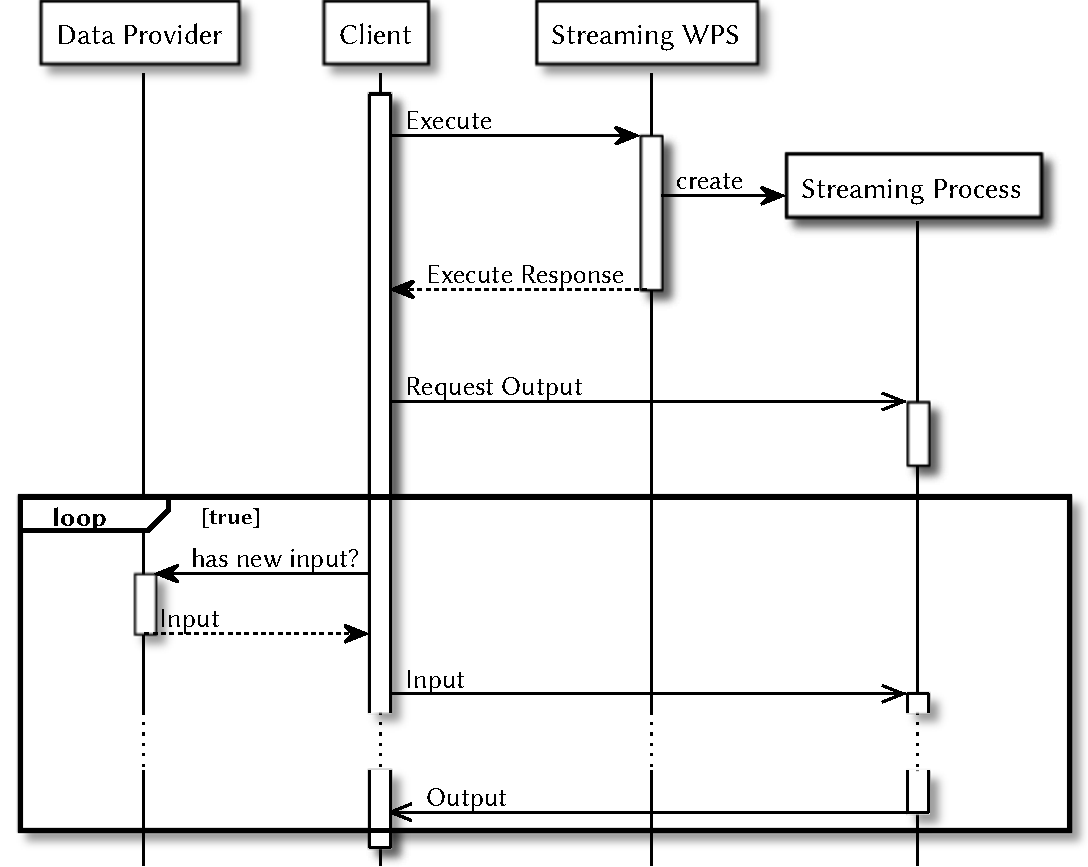
\includegraphics[width=.7868\textwidth]{figures/sequence-diagramm-polling.pdf}
				% 179x274
				\caption{\label{fig:sd:polling} Sequence diagram of how to implement polling inputs for a streaming enabled WPS algorithm.}
			\end{figure}

	\subsection{Dependencies}
		\label{sec:stream:dependencies}
		The definition of Reference Inputs in Section \ref{sec:stream:input:reference} implies a mechanism to resolve dependencies and to order the execution of streaming iterations. These are considered as tasks and can declare dependencies to other streaming iterations either by mapping an input to the output of another streaming iteration or by declaring a explicit dependency on another streaming iteration.

		Dependencies can be best modeled using a \ac{DAG}. A \ac{DAG} is a structure $D=(V, E)$ consisting of a set of vertices (or nodes) $V$ and edges (or arcs) $E$ where every edge $e\in E$ is a ordered pair $v_1 \rightarrow v_2$ with $v_1, v_2 \in V$. The distinct vertices $v_1,\dots,v_n\in V$ are called a path if for all successive vertices $v_i, v_{i+1}$ exists a edge $v_i \rightarrow v_{i+1} \in E$. A directed graph is called acyclic if there exists no path in $G$ with $v_1 = v_n$. A subgraph of a graph is the graph $G' = (V', E')$ with $V'\subseteq V$ and $E' = \{v_1 \rightarrow v_2 \in E | v_1, v_2\in V'\}$. Two subgraphs $G_1 = (V_1, E_1), G_2 = (V_2, E_2)$ are independent if $V_1 \cap V_2 = \emptyset$ and there exists no edge $v_1\rightarrow v_2\in E$ with $v_1\in V_1 \wedge v_2\in V_2$ or $v_2\in V_1 \wedge v_1\in V_2$.

		In a dependency graph, vertices represent a task, package or other entity that has dependencies and edges represent these dependencies ($v_1$ depends on $v_2$). Dependency graphs have to be acyclic as a cycle would introduce a cyclic dependency, that can not be resolved.

		\begin{figure}[!htb]
			\centering
			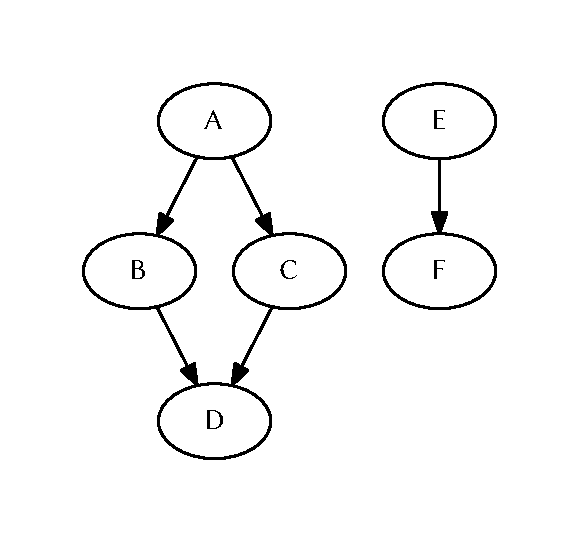
\includegraphics[width=.4474\textwidth]{figures/unordered-graph.pdf} % 98x92
			\caption{\label{fig:graph:unordered} Example for a dependency graph consisting of two independent subgraphs. Arrow denoting a dependency between the nodes.}
		\end{figure}

		A system containing the tasks $A, B, C, D, E, F$ and the dependencies $A\rightarrow B, A\rightarrow C, B\rightarrow D, C\rightarrow D$ and $E\rightarrow F$ will result in a \ac{DAG} consisting of two independent subgraphs (see Figure \ref{fig:graph:unordered}).

		The execution order of a dependency graph can be derived from the topological ordering of the graph: a ``topological ordering, $ord_D$, of a directed acyclic graph $D = (V, E)$ maps each vertex to a priority value such that $ord_{D}(x) < ord_{D}(y)$ holds for all edges $x \rightarrow y \in E$'' \citep{pearce2007dynamic}, a possible execution order is the list of all vertices sorted by descending $ord_D$. The topological order of a \ac{DAG} can be computed using e.g. \ac{BFS} in linear time \citep{cormen2001introduction}. In most cases the topological ordering is not unique, Figure \ref{fig:graph:ordered} shows one possible execution order for the before mentioned graph.

		\begin{figure}[!htb]
			\centering
			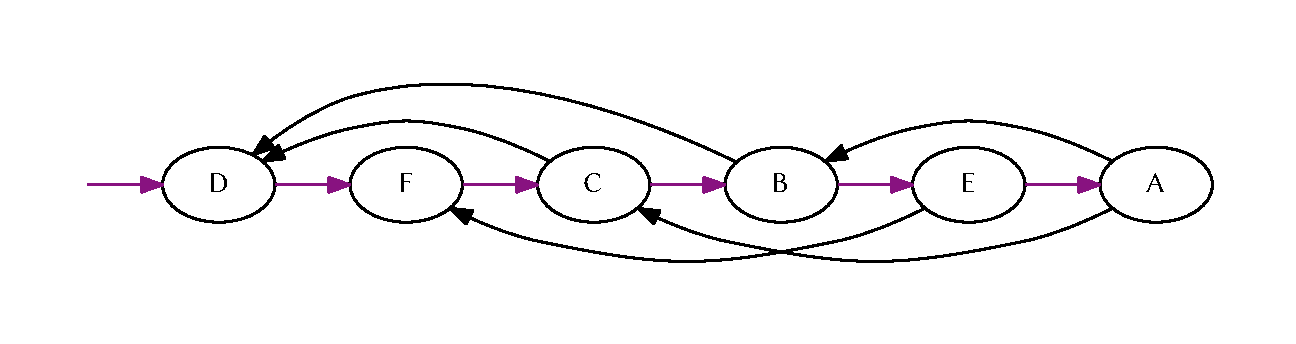
\includegraphics[width=1\textwidth]{figures/ordered-graph.pdf} % 219x58
			\caption{\label{fig:graph:ordered} Possible execution/topological order of the dependency graph in Figure \ref{fig:graph:unordered}. Black arrows represent dependence to another vertex, colored arrows the execution order.}
		\end{figure}

		In contrast to conventional dependency systems like package managers the Streaming \ac{WPS} can not operate on a static graph of dependencies but on a graph to which vertices and edges are added constantly. Conventional topological sorting algorithms have to recompute the ordering for every insertion from scratch which will have a big performance impact for the scenario of a great number of small streaming iterations. There exist few dynamic topological sort algorithms that will maintain the topological order across edge and node insertions and will only recompute the ordering if necessary.

		Most dependency graphs generated using the Streaming \ac{WPS} will probably consist of multiple independent subgraphs, no dependencies at all would be the most extreme example, or quite sparse graphs. For this the algorithm described by \citet{pearce2007dynamic} seems to be appropriate. Even it is theoretically it is inferior to other algorithms for dynamic topological sorting, it especially performs better on sparse graphs and on dense graphs only a constant factor slower than other algorithms \citep{pearce2007dynamic}. %wörtliches zitat?

		Dependencies are of particular importance in case of execution failures. If the computation of a streaming iteration fails for whatever reason, all iterations, that directly or indirectly depend on this iteration can not complete. As this also holds true for iterations, that are supplied at a later time in the streaming process, the process can not proceed ignoring the error. Due to this every error that occurs during the execution of a streaming iteration result in the termination of the streaming process.
		Dependencies also have a special meaning at the end of a streaming process, when a stop message is sent to notify the streaming process to accept no further inputs and finish pending streaming iterations. At this point all dependencies need to be able to be satisfied, which implies that all referenced input messages have been sent to the streaming process. In case a referenced input message the service is not able to complete gracefully and fail. As references to future streaming iterations are allowed, prior to this point, it is not possible for the Streaming \ac{WPS} to determine if reference may not be fulfilled. As the service is not able to fail fast for incorrect references, clients using dependencies between streaming iterations have to pay careful attention to references.

		It should also be noted, that the smallest referenceable unit for a streaming process is the output of a streaming iteration. Format specific references, e.g. to a particular feature inside a feature collection, are not possible using this protocol and streaming process implementations need to be designed to not need smaller components or have to deploy a own referencing strategy (e.g. by additionally supplying an additional input to identify the feature of the referenced collection). But, as this results in superfluous transfer of data, such solutions should be avoided. One may point out, that there is now way to reference input parameters of other streaming iterations, but this use case should be already covered by the \ac{WPS}' own input reference parameters (see section \ref{sec:streaming:input}).

	\subsection{Process Description}
		\label{sec:stream:processdescription}
		The conventional process description mechanism of the \ac{WPS} is not sufficient to describe streaming processes.

		It consists of a \texttt{DescribeProcess} request issued to the \ac{WPS} and the retrieval of one or more process descriptions of the specified process. These descriptions contain detailed descriptions of input and output parameters of the process and information about the supported formats, units of measurement or coordinate reference systems of each parameter. They also include details about allowed values, default value and multiplicity of input parameters \citep{ogc:wps}.

		Because the Streaming \ac{WPS} uses the \ac{WPS} interface only to start a Streaming Process and the \ac{WPS} interface does not provide any extension points for process descriptions, the \texttt{DescribeProcess} operation can only be used to describe the starting process, but not the input or output parameters of a streaming process.

		In case of generic processes, e.g. processes that delegate to other \ac{WPS} processes, information about input and output parameters is not even available prior to the execution of the streaming process. Furthermore input parameter cardinalities may change due to the use of static inputs. By this a valid input parameter for a delegate process may not be used in subsequent inputs because the maximal occurrence of the parameter is already exhausted using static input parameters. By this a process description for a streaming process will always be instance specific and can not be generated by the associated \ac{WPS} process.

		With knowledge of the delegate process a client may has enough information to facilitate the streaming process but for other streaming process there is no way for a generic client to know the input parameters of the process.

		To compensate this shortcoming a method is needed to describe a Streaming Process instance at runtime.
		\begin{itemize}
			\item other process description formats
			\item differentiation between intermediate results and final result
		\end{itemize}
	\subsection{WPS Specification Shortcomings}
	\begin{itemize}
		\item different procedure description format, like in the sensorweb
		\item process instance need to be identifiable
		\item WSDL like description language of wps processes
		\item differentiation between continous outputs and final results
		\item allow different transport layers (like websockets)
		\item allowing subsequent input parameters
	\end{itemize}
	\subsection{Implementation}
	\begin{itemize}
		\item Server:
		\begin{itemize}
			\item based on the 52°North WPS
			\item includeable module
			\item default implementation uses another WPS process as delegate
		\end{itemize}
		\item Client
		\begin{itemize}
			\item small JavaScript library
			\item abstracts the message generation and WebSocket interaction
			\item may be used to start generic delegation processes
		\end{itemize}
	\end{itemize}
	\subsection{Streaming Lake-Analyzer WPS}
	\begin{itemize}
		\item simple application of the Streaming WPS and \textsc{Matlab} WPS
		\item LakeAnalyzer may need further adjustments to allow live analysis
		\item remove down sampling code
		\item operate on single point in time
		\item etc
	\end{itemize}
	\subsection{Limitations}
	\begin{itemize}
		\item No input/output conversion
		\item Only default format is requested from delegate
		\item process will not fail fast in under every condition
		\begin{itemize}
			\item inputs first are checked at execution time
		\end{itemize}
		\item receivers are only provided with upcoming
		\begin{itemize}
			\item no replay queue
		\end{itemize}
	\end{itemize}
\section{Future Work}
\section{Conclusion}